\documentclass[polish,polish,a4paper]{article}
\usepackage{cmap}

\usepackage[T1]{fontenc}
\usepackage[utf8]{inputenc}
\usepackage{listings}
\usepackage{graphicx} 
\usepackage{tikz}
\usepackage{xcolor}
\usepackage{babel}
\usepackage{pslatex}
\usepackage{tikz}
\usepackage{pgfplots}
\usepackage{anysize}
\usepackage{pgfgantt}
\usepackage{latexsym,amsmath}

\marginsize{2.5cm}{2.5cm}{3cm}{3cm}
\graphicspath{ {D:\Nauka\Grafika Komputerowa\lab4 światło\latex} }


\title{Sprawozdanie nr 4}
\author{Łukasz Szumilas, Grupa E02-81o}
\date{Zajęcia: 17 grudnia 2018 (odrobione 20 grudnia)}

\begin{document}
  \begin{center}\Large
    Grafika Komputerowa i Komunikacja Człowiek-Komputer
  \end{center}
  \hrule
  {\let\newpage\relax\maketitle}
  \hrule


  \section{Omówienie tematu}
  Celem ćwiczenia była prezentacja możliwości oświetlenia obiektów 3D, a także jak można opisać własności materiału z którego jest wykonany oświetlany obiekt, jak na scenie zdefiniować źródło światła i jak dobrać jego parametry. Ukazano także sposób wyznaczania wektorów normalnych do punktów na powierzchni opisanej przy pomocy równań parametrycznych.
\\\indent Na początek, by przetestować wprowadzanie wśród obiektów 3D źródło światła, użyty był gotowy obiekt imbryczka, przywołany za pomocą funkcji  \textit{glutSolidTeapot()}. W funkcji \textit{MyInit()} dodane zostały fragmenty kodu przygotowane w instrukcji. Efekty widać na \textbf{\textit{kodzie nr 1, rysunku nr 1}}. By lepiej zobrazować padające światło, w pliku źródłowym zostały także dodane fragmenty kodu z poprzednich labolatoriów, pozwalające obracać obiekt z punktu widzenia potencjalnego obserwatora.
\\\indent Po wykonaniu tej części należało oświetlić już osobiście zdefiniowany obiekt. W tym przypadku było to jajko, kod potrzebny do jego wytworzenia został zaczerpnięty z owocnych starań na laboratorium o modelowaniu 3D. Efekt tego widnieje na \textbf{\textit{rysunku nr 2}}. Widać różnice w porównaniu z oświetlaniem imbryczka, które biorą się z braku informacji o wektorach normalnych do powierzchni. Takie współrzędne muszą zostać obliczone dla każdego punktu tworzącego jajko. 
 W \textbf{\textit{kodzie nr 3, rysunku nr 3}}, widać różnicę w oświetlaniu jajka po dodaniu takich wektorów. Jedyny mankament wynika z braku poprawnego odbicia wektorów normalnych po drugiej stronie modelu, co widać na rysunku. Aby to naprawić, wystarczy prosta instrukcja warunkowa przypisująca wartości przeciwne wektorom normalnym w sytuacji, gdy jesteśmy po drugiej stronie jajka \textbf{\textit{kod nr 4, rysunek nr 4}}.
 \\\indent Ostatnim etapem było dodanie drugiego źródła światła. Najważniejsze było poprawne operowanie składowymi intensywności świecenia, tak by dobrze było widać oba źródła. W \textbf{\textit{kodzie nr 5 i rysunku nr 5}} zostały dodane światła, czerwone i niebieskie. 
  \section{Omówienie kodu}
   \textbf{Kod 1}, fragment funkcji \textit{MyInit()}.
{\small
\begin{lstlisting}[language=C++]
//  Definicja materialu z jakiego zrobiony jest czajnik 
//  i definicja zrodla swiatla

// Definicja materialu z jakiego zrobiony jest czajnik 

    GLfloat mat_ambient[]  = {1.0, 1.0, 1.0, 1.0};        
    // wspolczynniki ka =[kar,kag,kab] dla swiatla otoczenia

    GLfloat mat_diffuse[]  = {1.0, 1.0, 1.0, 1.0};
    // wspolczynniki kd =[kdr,kdg,kdb] swiatla rozproszonego

    GLfloat mat_specular[] = {1.0, 1.0, 1.0, 1.0};
    // wspolczynniki ks =[ksr,ksg,ksb] dla swiatla odbitego                
    
    GLfloat mat_shininess  = {20.0};
    // wspolczynnik n opisujacy polysk powierzchnii

// Definicja zrodla swiatla
     GLfloat light_position[] = {0.0, 0.0, 10.0, 1.0};    
    // polozenie zrodla


    GLfloat light_ambient[] = {0.1, 0.1, 0.1, 1.0};
    // skladowe intensywnosci swiecenia zrodla swiatla otoczenia
    // Ia = [Iar,Iag,Iab]

    GLfloat light_diffuse[] = {1.0, 1.0, 1.0, 1.0};        
    // skladowe intensywnosci swiecenia zrodla swiatla powodujacego
    // odbicie dyfuzyjne Id = [Idr,Idg,Idb]

    GLfloat light_specular[]= {1.0, 1.0, 1.0, 1.0};
    // skladowe intensywnosci swiecenia zrodla swiatla powodujacego
    // odbicie kierunkowe Is = [Isr,Isg,Isb]

    GLfloat att_constant  = {1.0};
    // skladowa stala ds dla modelu zmian oswietlenia w funkcji 
    // odlgelosci od zrodla

    GLfloat att_linear    = {0.05}; 
    // skladowa liniowa dl dla modelu zmian oswietlenia w funkcji 
    // odlgelosci od zrodla

    GLfloat att_quadratic  = {0.001};
    // skladowa kwadratowa dq dla modelu zmian oswietlenia w funkcji
    // odlgelosci od zrodla

// Ustawienie parametrow materialu i zrodla swiatla

// Ustawienie parametrow materialu
    glMaterialfv(GL_FRONT, GL_SPECULAR, mat_specular);
    glMaterialfv(GL_FRONT, GL_AMBIENT, mat_ambient);
    glMaterialfv(GL_FRONT, GL_DIFFUSE, mat_diffuse);
    glMaterialf(GL_FRONT, GL_SHININESS, mat_shininess);

// Ustawienie parametrow zrodla

    glLightfv(GL_LIGHT0, GL_AMBIENT, light_ambient);
    glLightfv(GL_LIGHT0, GL_DIFFUSE, light_diffuse);
    glLightfv(GL_LIGHT0, GL_SPECULAR, light_specular);
    glLightfv(GL_LIGHT0, GL_POSITION, light_position);

    glLightf(GL_LIGHT0, GL_CONSTANT_ATTENUATION, att_constant);
    glLightf(GL_LIGHT0, GL_LINEAR_ATTENUATION, att_linear);
    glLightf(GL_LIGHT0, GL_QUADRATIC_ATTENUATION, att_quadratic);

// Ustawienie opcji systemu oswietlenia sceny 

    glShadeModel(GL_SMOOTH); // wlaczenie lagodnego cieniowania
    glEnable(GL_LIGHTING);   // wlaczenie systemu oswietlenia sceny 
    glEnable(GL_LIGHT0);     // wlaczenie zrodla o numerze 0
    glEnable(GL_DEPTH_TEST); // wlaczenie mechanizmu z-bufora 

\end{lstlisting}
}
\textbf{Kod 3}, funkcja tworzaca jajko z prawidlowo obliczonymi wektorami normalnymi po jednej stronie jajka.   
{\small
\begin{lstlisting}[language=C++]
	void Egg()
	{
	float numerU = 0;
	float numerV = 0;
	float distance = 1 / (N - 2);

	for (int i = 0; i < N; i++)
	{
		for (int j = 0; j < N; j++)
		{
		float u = numerU;
		float v = numerV;
		point2 a = { u,v };

		memcpy(UV[i][j], a, sizeof(a));

		float rownanieX = (-90 * pow(u, 5) + 225 * pow(u, 4)
		 - 270 * pow(u, 3) + 180 * pow(u, 2) - 45 * (u))*cos(3.14*(v));
		float rownanieY = (160 * pow(u, 4) - 320 * pow(u, 3) + 160 * pow(u, 2));
		float rownanieZ = (-90 * pow(u, 5) + 225 * pow(u, 4)
		 - 270 * pow(u, 3) + 180 * pow(u, 2) - 45 * (u))*sin(3.14*(v));
		point3 ej = { rownanieX, rownanieY, rownanieZ };

		memcpy(tabXYZ[i][j], ej, sizeof(ej));

			
		float xU = (-450 * pow(u, 4) + 900 * pow(u, 3) - 810 * 
		pow(u, 2) + 360 * (u)-45)*cos(3.14*(v));
		float xV = 3.14*(90 * pow(u, 5) - 225 * pow(u, 4) + 270 *
		 pow(u, 3) - 180 * pow(u, 2) + 45 * (u))*sin(3.14*(v));
		float yU = 640 * pow(u, 3) - 960 * pow(u, 2) + 320 * (u);
		float yV = 0;
		float zU = (-450 * pow(u, 4) + 900 * pow(u, 3) - 810 *
		 pow(u, 2) + 360 * (u)-45)*sin(3.14*(v));
		float zV = -3.14*(90 * pow(u, 5) - 225 * pow(u, 4) + 270 *
		 pow(u, 3) - 180 * pow(u, 2) + 45 * (u))*cos(3.14*(v));

		GLfloat first = yU * zV - zU * yV
		GLfloat second = zU * xV - xU * zV;
		GLfloat third = xU * yV - yU * xV;
		
		float vectorLength = sqrt((pow(first, 2)) + (pow(second, 2)) + (pow(third, 2)));

		first = first / vectorLength;
		second = second / vectorLength;
		third = third / vectorLength;


		point3 vectorNormal = { first,second,third };
		memcpy(tabVectorNormal[i][j], vectorNormal, sizeof(vectorNormal));
			

		if (i > 0 && j > 0) {
		glBegin(GL_TRIANGLES);
		glNormal3fv(tabVectorNormal[i - 1][j - 1]);
		glVertex3fv(tabXYZ[i - 1][j - 1]);

		glNormal3fv(tabVectorNormal[i - 1][j]);
		glVertex3fv(tabXYZ[i - 1][j]);

		glNormal3fv(tabVectorNormal[i][j]);
		glVertex3fv(tabXYZ[i][j]);
		glEnd();

		glBegin(GL_TRIANGLES);
		glNormal3fv(tabVectorNormal[i - 1][j - 1]);
		glVertex3fv(tabXYZ[i - 1][j - 1]);

		glNormal3fv(tabVectorNormal[i][j - 1]);
		glVertex3fv(tabXYZ[i][j - 1]);

		glNormal3fv(tabVectorNormal[i][j]);
		glVertex3fv(tabXYZ[i][j]);
		glEnd();
		}
		numerV += distance;
		}
	numerU += distance;
	numerV = 0;
	}
}
\end{lstlisting}
}
.\\
\textbf{Kod 4}, prosta instrukcja warunkowa pozwalająca poprawnie obliczyć wektory po drugiej stronie jajka.
{\small
\begin{lstlisting}[language=C++]
   if (u >= 0.5) {
		first *= -1;
		second *= -1;
		third *= -1;
	}
\end{lstlisting}
}



\textbf{Kod 5}, większa część kodu funkcji \textit{MyInit()}.
{\small
\begin{lstlisting}[language=C++]
GLfloat light_position[] = { -20.0, 0.0, 10.0, 1.0 };
	GLfloat light_position1[] = { 20.0, 0.0, 10.0, 1.0 };

	GLfloat light_ambient[] = { 0.1, 0, 0, 1.0 };
	GLfloat light_ambient1[] = { 0, 0, 0.1, 1.0 };

	GLfloat light_diffuse[] = { 1.0, 0, 0, 1.0 };
	GLfloat light_diffuse1[] = { 0, 0, 1.0, 1.0 };
	
	GLfloat light_specular[] = { 1.0, 1.0, 1.0, 1.0 };
	GLfloat light_specular1[] =  { 1.0, 1.0, 1.0, 1.0 };

	GLfloat att_constant = { 1.0 };
	GLfloat att_constant1 = { 1.0 };

	GLfloat att_linear = { static_cast<float>(0.05) };
	GLfloat att_linear1 = { static_cast<float>(0.05) };

	GLfloat att_quadratic = { static_cast<float>(0.001) };
	GLfloat att_quadratic1 = { static_cast<float>(0.001) };


	glMaterialfv(GL_FRONT, GL_SPECULAR, mat_specular);
	glMaterialfv(GL_FRONT, GL_AMBIENT, mat_ambient);
	glMaterialfv(GL_FRONT, GL_DIFFUSE, mat_diffuse);
	glMaterialf(GL_FRONT, GL_SHININESS, mat_shininess);


	glLightfv(GL_LIGHT0, GL_AMBIENT, light_ambient);
	glLightfv(GL_LIGHT0, GL_DIFFUSE, light_diffuse);
	glLightfv(GL_LIGHT0, GL_SPECULAR, light_specular);
	glLightfv(GL_LIGHT0, GL_POSITION, light_position);

	glLightf(GL_LIGHT0, GL_CONSTANT_ATTENUATION, att_constant);
	glLightf(GL_LIGHT0, GL_LINEAR_ATTENUATION, att_linear);
	glLightf(GL_LIGHT0, GL_QUADRATIC_ATTENUATION, att_quadratic);

	glLightfv(GL_LIGHT1, GL_AMBIENT, light_ambient1);
	glLightfv(GL_LIGHT1, GL_DIFFUSE, light_diffuse1);
	glLightfv(GL_LIGHT1, GL_SPECULAR, light_specular1);
	glLightfv(GL_LIGHT1, GL_POSITION, light_position1);

	glLightf(GL_LIGHT1, GL_CONSTANT_ATTENUATION, att_constant1);
	glLightf(GL_LIGHT1, GL_LINEAR_ATTENUATION, att_linear1);
	glLightf(GL_LIGHT1, GL_QUADRATIC_ATTENUATION, att_quadratic1);


	glShadeModel(GL_SMOOTH); 
	glEnable(GL_LIGHTING);   
	glEnable(GL_LIGHT0);     
	glEnable(GL_LIGHT1);    
	glEnable(GL_DEPTH_TEST); 
}
\end{lstlisting}
}

  \section{Rezultat prac}

    \begin{figure}[h!]
      \centering
      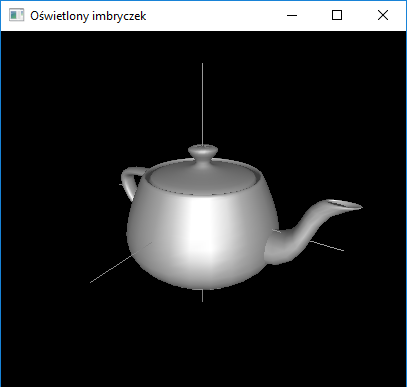
\includegraphics[width=0.6\textwidth,height=8cm]{imbryczek.png}
      \caption{Imbryczek. Oświetlenie.}
      \label{fig:zrzut1}
    \end{figure}

    \begin{figure}[h!]
      \centering
      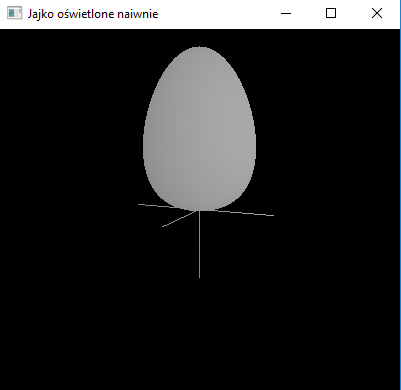
\includegraphics[width=0.6\textwidth,height=8cm]{jajkonaiwnie.png}
      \caption{Jajko oświetlone naiwnie.}
      \label{fig:zrzut1}
    \end{figure}

    \begin{figure}[h!]
      \centering
      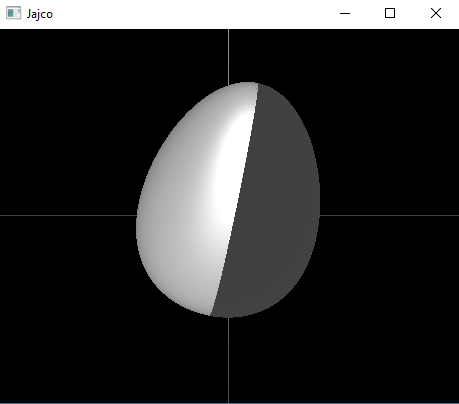
\includegraphics[width=0.6\textwidth,height=8cm]{jajkopolowka.png}
      \caption{Oświetlone jajko, zdefiniowane wektory normalne.}
      \label{fig:zrzut1}
    \end{figure}

    \begin{figure}[h!]
      \centering
      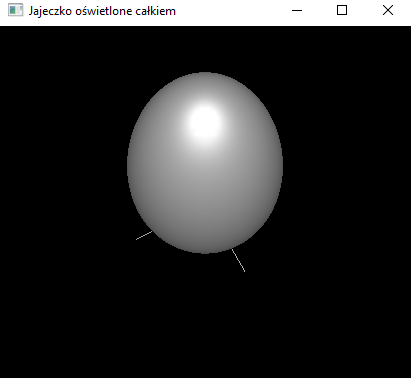
\includegraphics[width=0.6\textwidth,height=8cm]{jajkocale.png}
      \caption{Oświetlone jajko, poprawnie zdefiniowane wektory normalne.}
      \label{fig:zrzut1}
    \end{figure}
    
        \begin{figure}[h!]
      \centering
      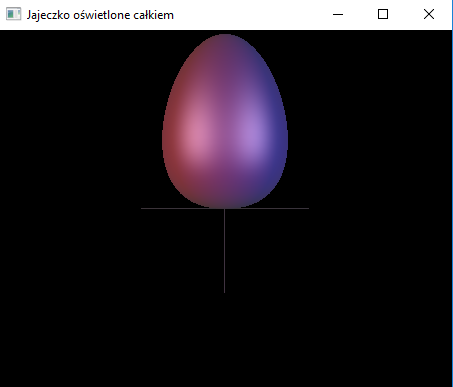
\includegraphics[width=0.6\textwidth,height=8cm]{jajkodwazrodla.png}
      \caption{Jajko oświetlone przez dwa źródła.}
      \label{fig:zrzut1}
    \end{figure}

\end{document}